% el problema
El problema del \textit{tráfico} que consideraremos tiene la siguiente premisa. Dado una ciudad representada por un conjunto $V$ de $n$ puntos conectados por un conjunto $E$ de $m$ calles unidireccionales, dos puntos críticos $s$ y $t \in V$, y un conjunto
\begin{equation*}
    P := \{p_1 \ ... \ p_k\}    
\end{equation*}
de $k$ calles bidireccionales candidatas, queremos saber cuál es la mínima distancia que deberemos recorrer para llegar de $s$ a $t$, dado que se construya una de estas calles.

Para ello, vamos a contar con la longitud $\ell^c_i$, $1 \leq i \leq m$ de cada calle en la ciudad y la longitud $\ell^p_j$, $1 \leq j \leq k$ de cada calle posible a construir.

Por ejemplo, si tuvieramos la siguiente ciudad ---cuyas calles candidatas están en color gris--- y los puntos críticos $s = 1$ y $t = 4$

\begin{figure}[!htbp]
    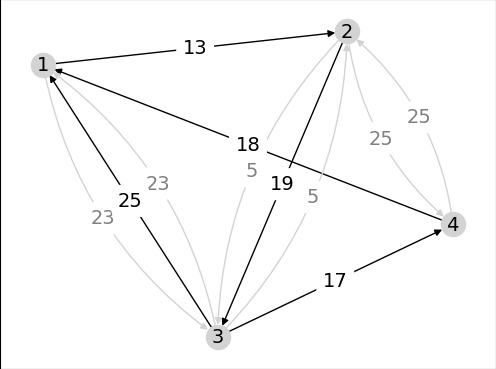
\includegraphics[scale=0.5, trim={0.2cm 0.2cm 0.2cm 0.2cm}, clip]{/files/src/.media/grafo.png} 
    %\caption{s} \label{ejemplo}
\end{figure}
    
\noindent entonces podríamos construir la calle $2 \leftrightarrow 3$ de longitud $5$ para lograr un recorrido mínimo $1 \to 2 \to 3 \to 4$ de largo $35$.

% modelado
\subsection{Modelado como un problema de camino mínimo}\label{modelo} 

A partir del ejemplo anterior, vemos que el problema del \textit{tráfico} se puede modelar de manera intuitiva como un problema de \textit{camino minimo} en grafos: sea $D$ el digrafo asociado a una ciudad $(V,\ E)$ y sea $w: E \to \mathbb{R}_{+}$ una función de peso, donde $w(c_i) = \ell^c_i$, $c_i \in E$ para todo $1 \leq i \leq m$, y $w(p_i) = \ell^p_i$, $p_i \in P$ para todo $1 \leq i \leq k$. Luego, podemos resolver el problema del \textit{tráfico} si evaluamos el mínimo entre todos los caminos mínimos entre $s$ y $t$ para cada digrafo en la sucesión
\begin{equation}\label{eq_1}
    \{D\} \cup \{(V,\ E \cup \{e,\ \bar{e}\}) : e \in P\}
\end{equation}
utilizando la función de peso $w$.

Sin embargo, esto no es eficiente. De emplear el algoritmo de \textit{Dijkstra} con \textit{min-heap}, la complejidad de peor caso estaría en $O(k\cdot m\log n)$. Vamos a ver cómo lo podemos mejorar. 

% algoritmo
\subsection{El algoritmo}

Notar primero que el camino mínimo entre dos vértices $s$ y $t$ satisface la propiedad de \textit{subestructura óptima}\footnote{Ver Cita \ref{foot_1}, sección 16.2: \textit{Elements of a greedy strategy}.}. Esto es, cada sección del camino forma, a su vez, un camino mínimo\footnote{Si no, podríamos reemplazar esta sección por otra de menor distancia, lo que es una contradicción.}. 

Sigue que, si $\delta_D : E \to \mathbb{R}$ es la distancia mínima entre cualquier par de vértices en un digrafo $D = (V,\ E)$ con función de peso $w: E \to \mathbb{R}$ que no tiene ciclos negativos, entonces para cualquier par de vértices $s$ y $t$ en $V$, para los cuales existe un camino $s \rightsquigarrow t$, y una arista $(u,\ v)$ perteneciente a este camino, $\delta_D(s,\ t) = \delta_D(s,\ u) + w(u,\ v) + \delta_D(v,\ t)$.

Vamos a demostrar en la siguiente sección que una consecuencia de esta observación es que, de agregar una arista $e = (u,\ v)$ a $D$ con peso $\ell$ no negativo, entonces 
\begin{equation}\label{eq_2}
    \delta_{D + e}(s,\ t) = \min\{\delta_{D}(s,\ u) + \ell + \delta_{D}(v,\ t),\ \delta_{D}(s,\ t)\}.
\end{equation}

En particular, dado que $\delta_D(s,\ t) = \delta_{D^t}(t,\ s)$\footnote{ Notar que los caminos en un digrafo son \textit{dirigidos}. Luego, las distancias son simétricas respecto al digrafo transpuesto.} y que nuestro problema se restringe a pesos no negativos, estas observaciones nos permiten considerar el siguiente algoritmo.

\lstinputlisting[mathescape=true, language=pseudo, label=trafico, caption={Pseudocódigo para el problema del \textit{tráfico}.}]{files/src/.code/trafico.pseudo}

El mismo aplica un algoritmo de \textit{camino mínimo con única fuente} sobre el grafo de entrada $D$, a partir de $s$, y sobre el grafo transpuesto $D^t$, a partir de $t$, para saber la distancia mínima ---que se guarda en los diccionarios $\delta^s$ y $\delta^t$--- de ambos vértices a todo el resto de los vértices en el digrafo. Luego, aplica la ecuación \ref{eq_2} para determinar cuál es la distancia mínima entre $s$ y $t$ en cada par de digrafos $(D + e,\ D + \bar{e})$\footnote{Esto es equivalente a considerar el digrafo $D + \{e,\ \bar{e}\}$, ya que ambas aristas no pueden pertenecer a un mismo camino mínimo. Esto se debe a que, si ambas aristas pertenecieran en simultáneo, formarían un ciclo.} para cada calle bidireccional $e$ en $P$.

% correctitud
\subsection{Demostración de correctitud}\label{correctitud}  

Dada la discusión anterior, basta demostrar que la ecuación \ref{eq_2} se satisface para demostrar que el algoritmo \ref{trafico} encuentra la distancia del camino mínimo entre $s$ y $t$ dentro del conjunto de digrafos definido por la ecuación \ref{eq_1}.

\begin{proof} 
    Sea $D$ un digrafo $D = (V,\ E)$ con función de peso $w: E \to \mathbb{R}$ que no tiene ciclos negativos y sea  $\delta_G : E \to \mathbb{R}$ la distancia mínima entre cualquier par de vértices en un digrafo $G$ cualquiera.

    Consideremos el digrafo $D+e$, con $e = (u,\ v)$, tal que $e$ es una arista entre dos vértices de $V$ que no está en $D$ y tiene peso $\ell$ no negativo. 
    
    Si $e$ no pertenece a ningún camino mínimo de $s$ a $t$ en $D + e$, sigue trivialmente que $\delta_{D + e}(s,\ t) = \delta_{D}(s,\ t)$, ya que $D \subset D + e$. Si, en cambio, sí pertenece, entonces debe ser que
    \begin{equation*}
        \delta_{D + e}(s,\ t) \leq \delta_{D}(s,\ t)
    \end{equation*} 
    ya que, o bien $e$ \textit{mejora} el camino mínimo entre ambos vértices, o bien lo mantiene igual, pero no puede suceder que lo empeore. Si no, dado que cualquier camino mínimo en $D$ está en $D + e$, el camino que contiene a $e$ no sería mínimo. 
    
    Del resultado anterior, y por la propiedad de \textit{subestructura óptima} del camino mínimo, sigue que
    \begin{equation}\label{eq_3}
        \delta_{D + e}(s,\ t) = \begin{cases}
            \delta_{D + e}(s,\ u) + \ell + \delta_{D + e}(v,\ t) &\text{si}\ e \in\ C_{st}(D+e)\\
            \delta_{D}(s,\ t) &\text{si no}
        \end{cases}
    \end{equation}
    donde $C_{st} \subset D + e$ es el subgrafo de caminos mínimos entre $s$ y $t$.

    Dado que cualquier camino mínimo de $s$ a $u$ y cualquier camino mínimo de $v$ a $t$ en $D + e$ no puede contener a la arista $e$ ---ya que, si no, se formaría un ciclo---, podemos concluir que $ \delta_{D + e}(s,\ u) = \delta_{D}(s,\ u) $ y $ \delta_{D + e}(v,\ t) = \delta_{D}(v,\ t)$. En particular, sigue que la ecuación \ref{eq_3}, es equivalente a
    \begin{equation*}
        \delta_{D + e}(s,\ t) = \min\{\delta_{D}(s,\ u) + \ell + \delta_{D}(v,\ t),\ \delta_{D}(s,\ t)\}.
    \end{equation*}
\end{proof}
    
% complejidad
\subsection{Complejidad temporal y espacial}

El algoritmo \texttt{trafico} depende casi exclusivamente de la implementación de \textit{camino mínimo} que utilicemos. %Considerando que puede haber diferentes valores para los pesos de las aristas no podemos hacer BFS, y como no se sabe si en el grafo hay ciclos, tampoco se puede usar el algoritmo de orden topológico. Estos dos resultan eficientes si se garantizan sus respectivas precondiciones. 
Dado que no tenemos garantias sobre la estructura del grafo de entrada\footnote{En particular, las longitudes pueden ser distintas ---lo que descarta el uso de \textit{BFS}--- y el digrafo no es necesariamente acíclico ---lo que descarta el uso del algoritmo de orden topológico---.}, más allá de que el peso de las aristas es no negativo, la mejor\footnote{ En base a los algoritmos conocidos.} complejidad que podemos lograr corresponde a utilizar el algoritmo de \textit{Dijkstra} sobre una estructura de \textit{fibonacci-heap}. El costo temporal resultante es $\Theta(k + m + n\log n)$, correspondiente a la construcción del digrafo de entrada y su transpuesta, dos invocaciones de \textit{Dijkstra} y las $k$ iteración del ciclo que comienza en la línea $5$ del algortimo \ref{trafico}. Por su parte, el costo espacial es $\Theta(m + n)$, correspondiente a las estructuras de los digrafos y el costo espacial de \textit{camino mínimo}.  %cuyo costo espacial es $\Theta(n)$ y cuyo costo temporal es $\Theta(m + n\log n)$\footnote{Ver cita \ref{foot_1}, sección 24.3.}. Luego, nuestro problema resultaría en una complejidad temporal en $\Theta(k + m + n\log n)$, correspondiente a la construcción del digrafo de entrada y su transpuesta, dos invocaciones de \textit{camino mínimo} y las $k$ iteración del ciclo que comienza en la línea $5$. El costo espacial estaría en $\Theta(m + n)$, correspondiente a las estructuras de los digrafos y el costo espacial de \textit{camino mínimo}. 
